\chapter{Evaluation}
\label{ch:evaluation}

This chapter describes the experiments conducted to evaluate the RFID hardware and localisation accuracy of the system. Each experiment description consists of justification, setup, results, and analysis. Section \ref{sec:hardeval} presents tests of the RFID hardware that provide an understanding of the mapping between RSSI and distance. Then, section \ref{sec:syseval} details the experiments that check whether the problem, described in section \ref{sec:probdef}, is solved by the system. It also provides results in terms of localisation accuracy and how these compare to results of the related work.

\section{Hardware Evaluation}
\label{sec:hardeval}

This section presents the experiments conducted in attempt to correlate received signal strength indicator (RSSI) and distance. This was accomplished by positioning the RFID tag at increasing distances and recording RSSI measurements from the RFID readers. Distance measurements were marked by a tape measure and RSSI values were recorded using the \textsf{SerialConnection} class, described in section \ref{sec:constread}. All experiments had taken place in two indoor environments, an apartment and a university computer laboratory. These places differ in the amount of open space and the number and placement of objects.

In indoor environments, the attenuation of a radio signal is strongly influenced by the physical effects of reflection, refraction, multipath and shadow fading. Following from that, in order to construct a more complete notion of the relationship between RSSI and distance, a number of experiments were carried out. These include how RSSI changed as distance increased at different orientations of the tag to the readers and elevations of the tag from the floor. In addition, the wall penetration and range capabilities of the hardware were evaluated. The following subsections describe these experiments.

\subsection{Range}
\label{subsec:range}

The aim of this experiment was to measure the range capabilities of the RFID equipment in an indoor environment. In addition, RSSI values were recorded as distance between the readers and tag increased. The devices were keeping a line of sight between each other. Then, the test was repeated by obscuring the tag with an object, in this case a large whiteboard, to determine if it was affecting the communication range of the devices and the RSSI values reported by the readers. The experiments were carried out for each of the readers in a computer laboratory that had a 13-meter-long stretch of open space. The results of these experiments are illustrated on Figure \ref{fig:13m}.

\begin{figure}[h]
	\begin{center}
		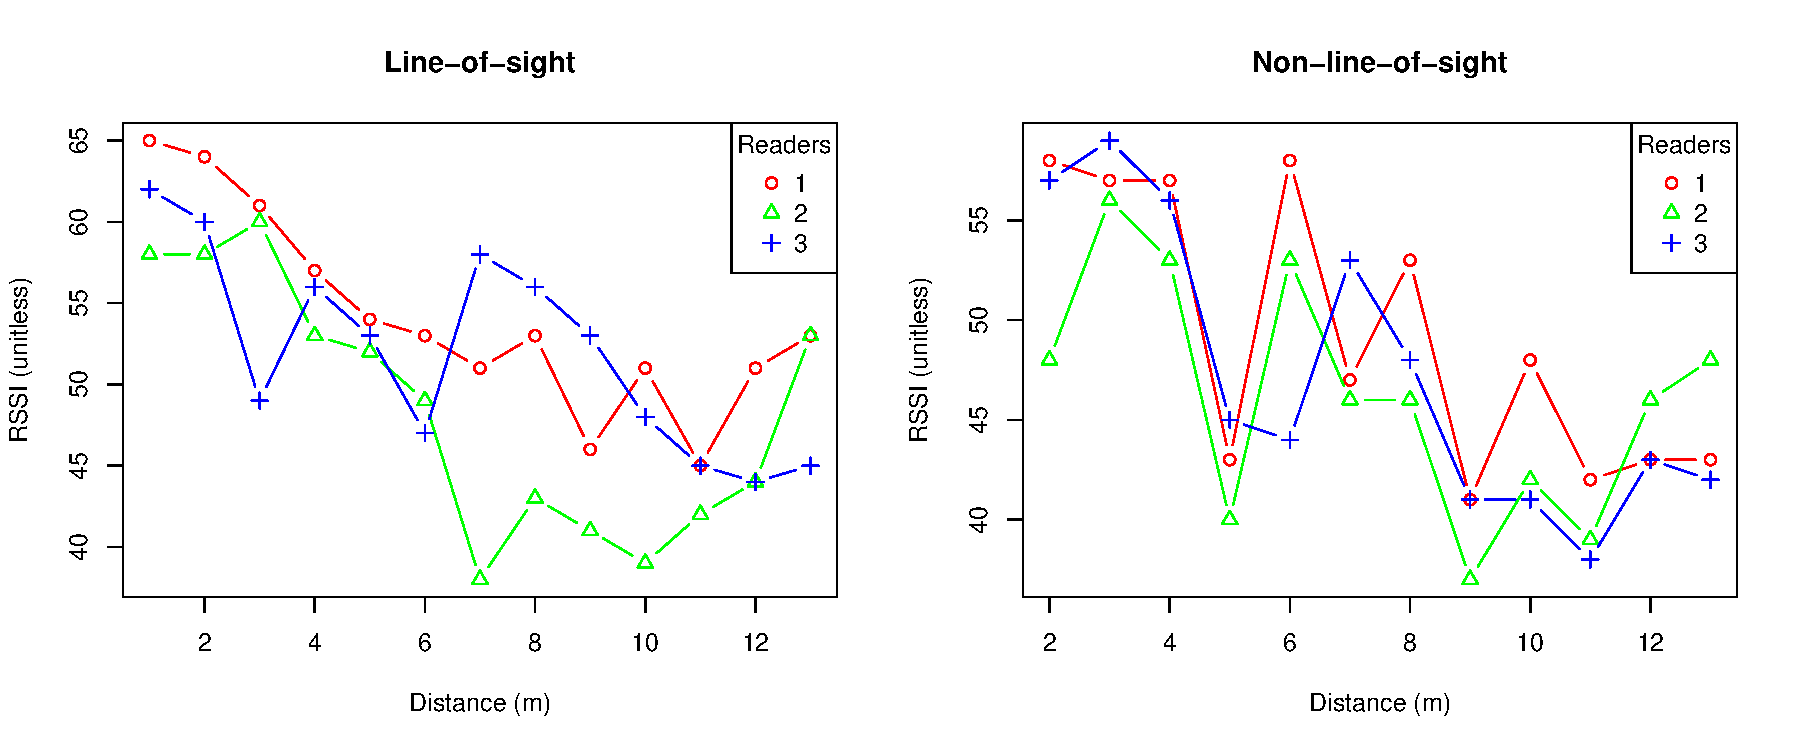
\includegraphics[width=1\textwidth]{figures/rssi_distance_13m}
		\caption{Two plots of RSSI measurements at increasing distances. On the $x$-axis, the distances from one to 13 meters are shown. The $y$-axis is the RSSI range. Notice how the RSSI ranges differ between the plots. The left graph shows RSSI value changes with a line-of-sight signal propagation between devices. The right graph illustrates the same experiment but with a non-line-of-sight signal propagation, that is the tag was occluded by an object.}
		\label{fig:13m}
	\end{center}
\end{figure}

Three observations could be made by looking at the above results. First, in both experiments all three readers were able to detect the tag when located 13 meters away. The manufacturer reported a transmission range of 8 meters. Consequently, the antenna, designed in this project, had definitely increased the transmission range of the RFID tag. 

Second, these experiments confirm that the readers measure different RSSI at equal distances. As distance increases, the average difference of RSSI values is 4.93. RSSI ranges on the $y$-axis are between 20 and 30. Following from that, if the measurements reported by the readers differ in an average of around five units given the above ranges, then these readers are not calibrated to each other. This was observed in subsequent experiments as well. It was the motivation for constructing separate translation tables when mapping RSSI to distance.

Third, it is known that radio signals suffer from the effects of various physical phenomena when propagating in indoor environments. Figure \ref{fig:13m} shows that RSSI measurements do not decrease steadily and often fluctuate as the distance increases. This could be contributed to the characteristics of indoor spaces, where the shape of the space and the objects in it could cause reflection, refraction, and absorption of radio signals. Introducing an object that occluded the RFID tag had definitely decreased the RSSI values reported by the readers. It also caused the measurements to vary in unexpected ways.


\subsection{Orientation of tag to reader}

This experiment investigated whether placing the tag at different positions around the readers, would affect RSSI measurements as distance increases. Outcomes of this test contributed to the understanding of the factors that determine how RSSI changes in different cases. The experiment started by placing the tag so that it touched antennas with a reader. Then, the tag was moved away at half a meter marks until the distance was three meters. Next, the tag was rotated counterclockwise around a reader at 45-degree steps. The experiment was done for each reader. In addition, the tests were repeated by placing a filled suitcase in front of the tag to simulate the tag being carried by a human or attached to an object. The concept of the experiments is illustrated on Figure \ref{fig:ori}.
\begin{figure}[h]
	\begin{center}
		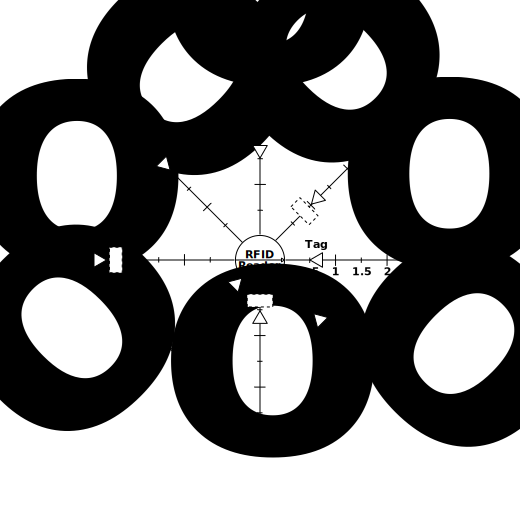
\includegraphics[width=.5\textwidth]{figures/exp/orientation}
		\caption{Examples positions of the tag and obstacle around one of the readers.}
		\label{fig:ori}
	\end{center}
\end{figure}

The results from the experiments are illustrated on Figures \ref{fig:oril} and \ref{fig:orin}. Figure \ref{fig:oril} shows the changes in RSSI as distance increases for different orientations of the tag with respect to the first reader in a line-of-sight radio propagation. Figure \ref{fig:orin} is a plot of a similar experiment but with the tag being obscured by an object. Notice that the minimum distance between devices is half a meter, which is needed to place the obstacle. Plots of the results using the other two readers are shown in Appendix \ref{sec:oriap}.
\begin{figure}[H]
	\begin{center}
		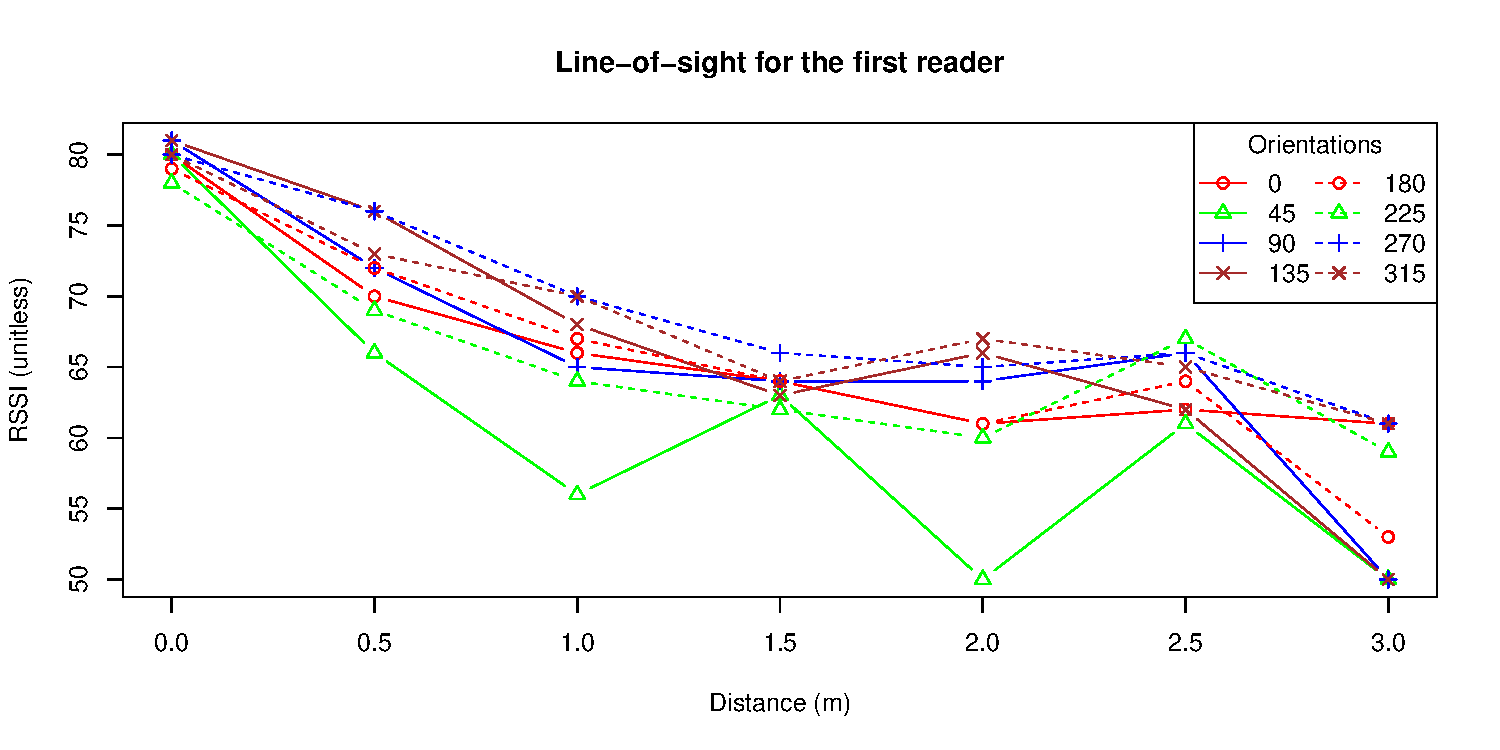
\includegraphics[width=1\textwidth]{figures/rssi_distance_3m_los_r1}
		\caption{Plot of RSSI measurements of different orientations of the tag with respect to the first reader. There was  a line of sight between the RFID devices.}
		\label{fig:oril}
	\end{center}
\end{figure}

The first thing to notice is that when the tag touches antennas with any of the readers, they reported RSSI values of around 80 units. This was unfortunate because the manufacturer had advertised an RSSI resolution from zero to 255. Clearly, the maximum values were much lower, which certainly had an impact on the localisation accuracy of the system. Nevertheless, the aim of the experiment was different. It tried to test whether the position of the tag around any of the readers had any significance on the measured received signal strength indicator. Figure \ref{fig:oril} is hard to follow but it is evident that regardless of the orientation of the tag, the first reader had measured similar RSSI values as distance increased. There are some points that lie outside of the main areas of values, which might be attributed to physical conditions in the indoor environment or in voltage variations in the battery of the tag. Another observation is that along opposite orientations of the tag, such as 90 and 270 degrees, measurements follow similar paths and have small differences in their RSSI values. This had no real significance for this project but is surely a pattern that could be spotted. 
\begin{figure}[h]
	\begin{center}
		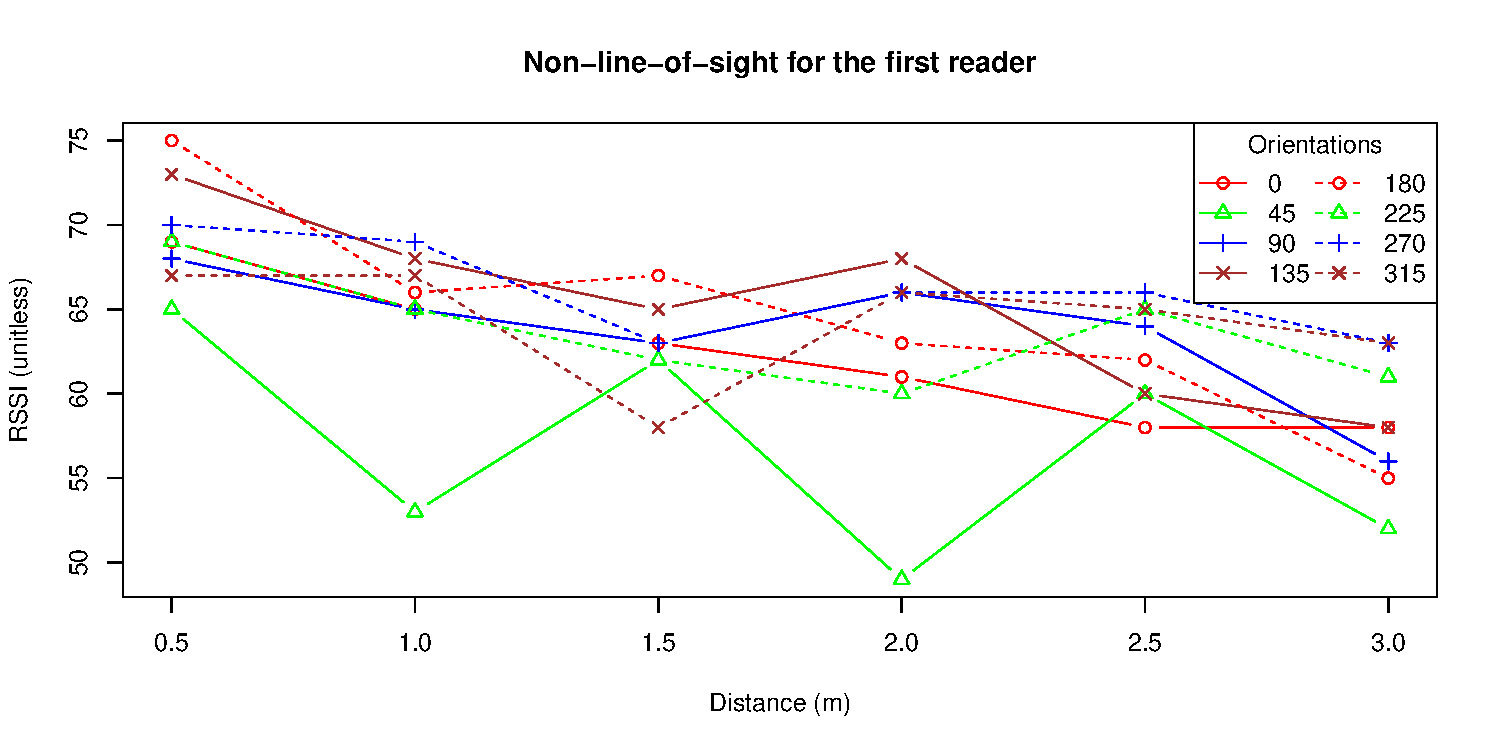
\includegraphics[width=1\textwidth]{figures/rssi_distance_3m_nlos_r1}
		\caption{Plot of RSSI measurements of different orientations of the tag with respect to the first reader. The tag was obscured by an object.}
		\label{fig:orin}
	\end{center}
\end{figure}

As explained above, the experiment was repeated by positioning an object in front of the tag to determine the impact of such occlusion on the RSSI measurements. Similar to the range experiments in section \ref{subsec:range}, lower RSSI values were recorded at close distances but the overall range of values on Figure \ref{fig:orin} is very similar to the one in the previous experiment. In contrast, RSSI measurements are more spread out at most distances, which is an indication that obstructing bodies do have an effect on the amount at which RSSI varies.


\subsection{Grid of positions}

The purpose of this experiment was to obtain further information on the relationship between RSSI and distance. More specifically, it was checked how RSSI would change when the tag was rotated around itself while being moved on a four by four grid of positions. Each reader was placed at the upper left corner (\verb!position(0,0)!) and the distance between adjacent points on the grid was one meter. The tag was rotated at 90 degree intervals starting by facing the right side of the grid. The results from this experiment using the first reader are shown on Figure \ref{fig:rssigrid}. Results obtained from the other readers are plotted in Appendix \ref{sec:rssigridap}.
\begin{figure}[H]
	\begin{center}
		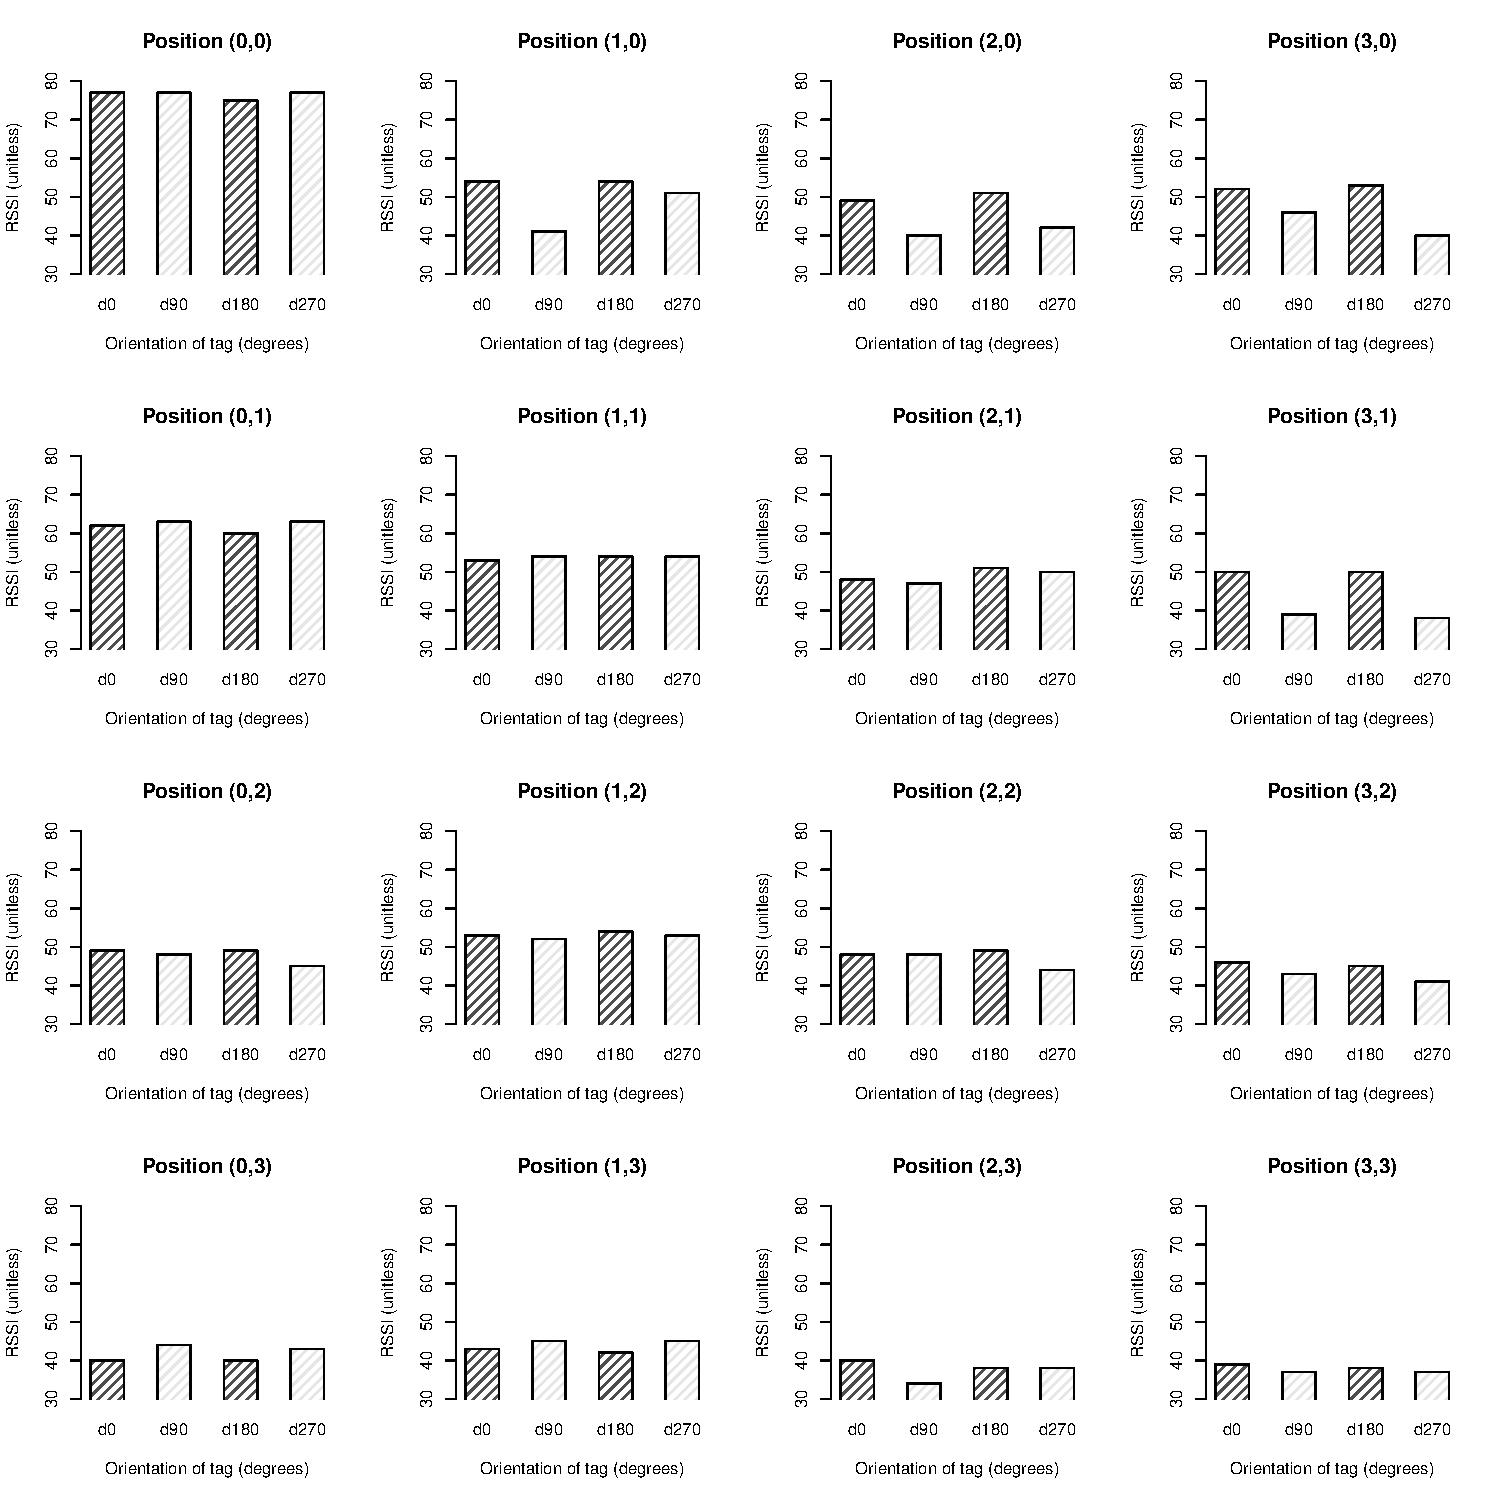
\includegraphics[width=1\textwidth]{figures/rssi_distance_grid_r1}
		\caption{Sixteen plots organised into a four by four grid. Each plot represents the RSSI measurements of the \textbf{first} reader when the tag was placed at different positions on the x and y axes of the grid. The positions of the tag were  measured in meters. The four bars in each plot show the RSSI readings when the tag was facing right (0\textdegree), up (90\textdegree), left (180\textdegree), and down (270\textdegree).}
		\label{fig:rssigrid}
	\end{center}
\end{figure}

Using the knowledge obtained from previous experiments, the range of RSSI values on the $y$-axis was limited between 30 and 80 RSSI. In this way, the differences in the measurements from various tag orientations are easier to spot. It also tells the reader that there were around 50 units of resolution provided by the RSSI module of the RFID readers. The manufacturer had claimed 256 steps of RSSI sensitivity, which was never achieved in this project. The leftmost column on Figure \ref{fig:rssigrid} illustrates the change in RSSI when the tag was placed in front of the reader. It can be seen that regardless of the rotation of the tag around its base, the RSSI values gradually drop. In contrast, the top row contains bar plots showing the tag being moved to the right of the reader. When it was facing up (90\textdegree) and down (270\textdegree), the tag was detected with up to 10 units less than in the other two orientations. The reason for this might have been that the radio waves emitted by the tag had to first bounce of walls or objects before being received by the reader. The conclusion that can be made is that although the devices were situated only one to three meters away, certain orientations of the tag might be perceived by the reader as the tag being further that it really was. Consequently, the orientation of the tag had an impact in some cases, which ultimately influences the localisation accuracy of the system.


\subsection{Elevation from floor}

The aim of this experiment was to investigate how RSSI would change if the tag was positioned at different heights relative to the room floor. The readers were placed at 6, 60, and 130 centimetres from the ground. Measurements were taken at these heights as the distance between the devices increased from one to four meters in half a meter steps. The setup of this experiment is illustrated on Figure \ref{fig:ele}.
\begin{figure}[h]
	\begin{center}
		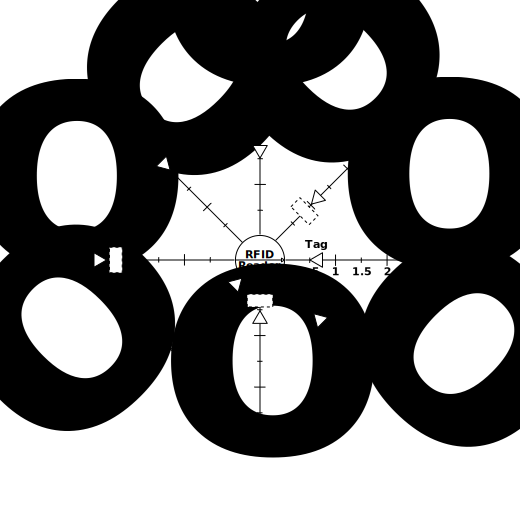
\includegraphics[width=.4\textwidth]{figures/exp/elevation}
		\caption{Positions of the tag when being elevated from the floor as distance increased. The readers were located at 6, 60, and 130 centimetres from the floor.}
		\label{fig:ele}
	\end{center}
\end{figure}

Experimental results can be seen on Figure \ref{fig:eler}. Each plot represents the RSSI measurements of the three readers with the tag being elevated at a specific height from the floor. On the first plot, the tag is very close to the ground (6cm). Logically, the third reader, which is also at the same height, generally measured higher RSSI values as the tag was being moved away. The other readers scored similar results with certain fluctuations in the measurements, which might be caused by the batteries, motion in the indoor environment, or simply by the quality of the devices. Similar trends are observed in the other two plots. It is interesting to note that as the tag is elevated higher in a room, reader measurements become more stable and large variations occur less often. An explanation might be that the upper parts of indoor spaces are usually free from obstacles, which provides a more reliable propagation medium.
\begin{figure}[H]
	\begin{center}
		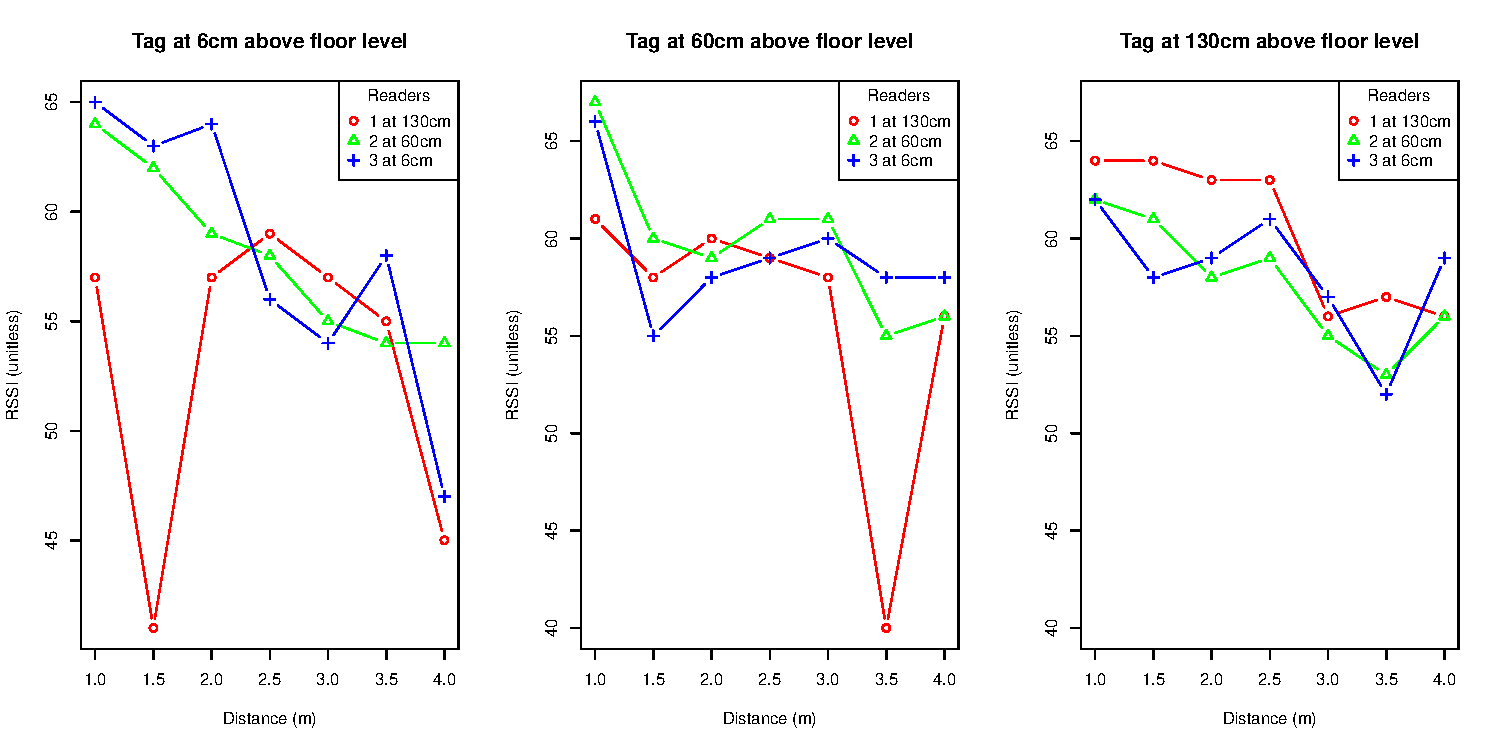
\includegraphics[width=1\textwidth]{figures/rssi_distance_4m}
		\caption{Three plots of RSSI measurements at increasing distances with the readers at different elevation from the floor. The first graph shows readings when the tag is placed 6cm above the floor level. The second and third graph show the same experiment but the tag is at 60cm and 130cm from the ground.}
		\label{fig:eler}
	\end{center}
\end{figure}


\subsection{Wall penetration}

This last experiment of the RFID hardware involved testing the wall penetration capabilities of the radio signal emitted from the tag. The setup for this test is shown on Figure \ref{fig:pene}. One of the readers was placed in a room. The tag was first positioned in the adjacent room and reported 41 RSSI. Then, it was moved in the next room, where it was detected with 51 and 40 RSSI in the nearest and furthest points of this space. Finally, the transmitter was carried outside the building. The reader was being able to detect it through two thinner inside and one thicker outside walls. This experiment was conducted to get an idea of the range capabilities of these RFID devices. This simple test showed that if the readers are positioned in different rooms they might be able to detect transmitters. 
\begin{figure}[h]
	\begin{center}
		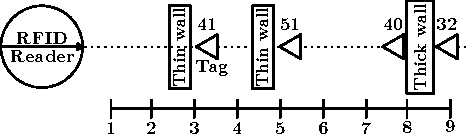
\includegraphics[width=.6\textwidth]{figures/exp/penetration}
		\caption{Experimental setup of the wall penetration test. The tag was positioned at 3, 4.8, 7.5, and 8.6 metres from one of the readers. The numbers above the tag are the measured RSSI.}
		\label{fig:pene}
	\end{center}
\end{figure}


\section{System evaluation}
\label{sec:syseval}

This section presents the experiments conducted to test the localisation system developed in this project. They tried to check the hypothesis, which is to evaluate the possibility of building a system capable of estimating the position of an unknown object with a certain accuracy using affordable RFID equipment and Raspberry Pi computers. The results of these experiments consist of the errors in meters between the computed and real positions of the tag. At the end of this chapter, the average localisation error is compared to the results of the related work. The following subsections describe the experiments carried out to evaluate this system.


\subsection{Grid of positions with line-of-sight propagation}

The aim of this experiment was to investigate the performance of the system when all readers had a line of sight to the tag and the devices were lying on the same plane, thus working in two dimensions. This was the case where the system was expected to output its best results because the setup had omitted obstacles sitting in between the devices. A grid of 16 positions was marked on the floor of an indoor space. The distance between any of the adjacent points was one meter, hence forming a three by three meter square. The RFID readers were positioned at the upper left, upper right, and bottom left corners of the grid. These were positions (0,0), (3,0), and (0,3) if all points of the grid had coordinates starting from the upper left corner with $x$ positive to the right and $y$ positive down. The tag was consequently placed in all positions. In addition, it was rotated around itself at 90 degree steps. This was done check if the orientation of the tag had an impact on the accuracy of the system. For every orientation, the localisation error in $x$ and $y$ was recorded.
\begin{figure}[H]
	\begin{center}
		
\includegraphics[width=1\textwidth]{figures/error_distance_grid}
		\caption{Sixteen plots are organised into a four by four grid. The readers are placed at positions (0,0), (3,0), and (0,3). Each plot represents the error in meters between measured and estimated location when the tag is placed at different positions on the grid. Each plot consists of four ellipses that illustrate the x and y error when the tag is facing right (0\textdegree), up(90\textdegree), left (180\textdegree), and down (270\textdegree). The colours of the ellipses are red, green, blue, and black, respectively.}
		\label{fig:errorlos}
	\end{center}
\end{figure}

Figure \ref{fig:errorlos} illustrates the results of this experiment. Every position of the grid is represented as a plot of the error in $x$ and $y$ for the four possible orientations. The centres of the plots mark a zero localisation error. Errors are drawn as ellipses that are stretched in the direction of the error. Different colours label the orientation of the tag when the measurements were recorded. For instance, when the tag was at position (1,3) and was looking to the right (0\textdegree), the error, coloured in red, was around two and half meters in $x$ and around a meter in $y$. 
\begin{figure}[H]
	\begin{center}
		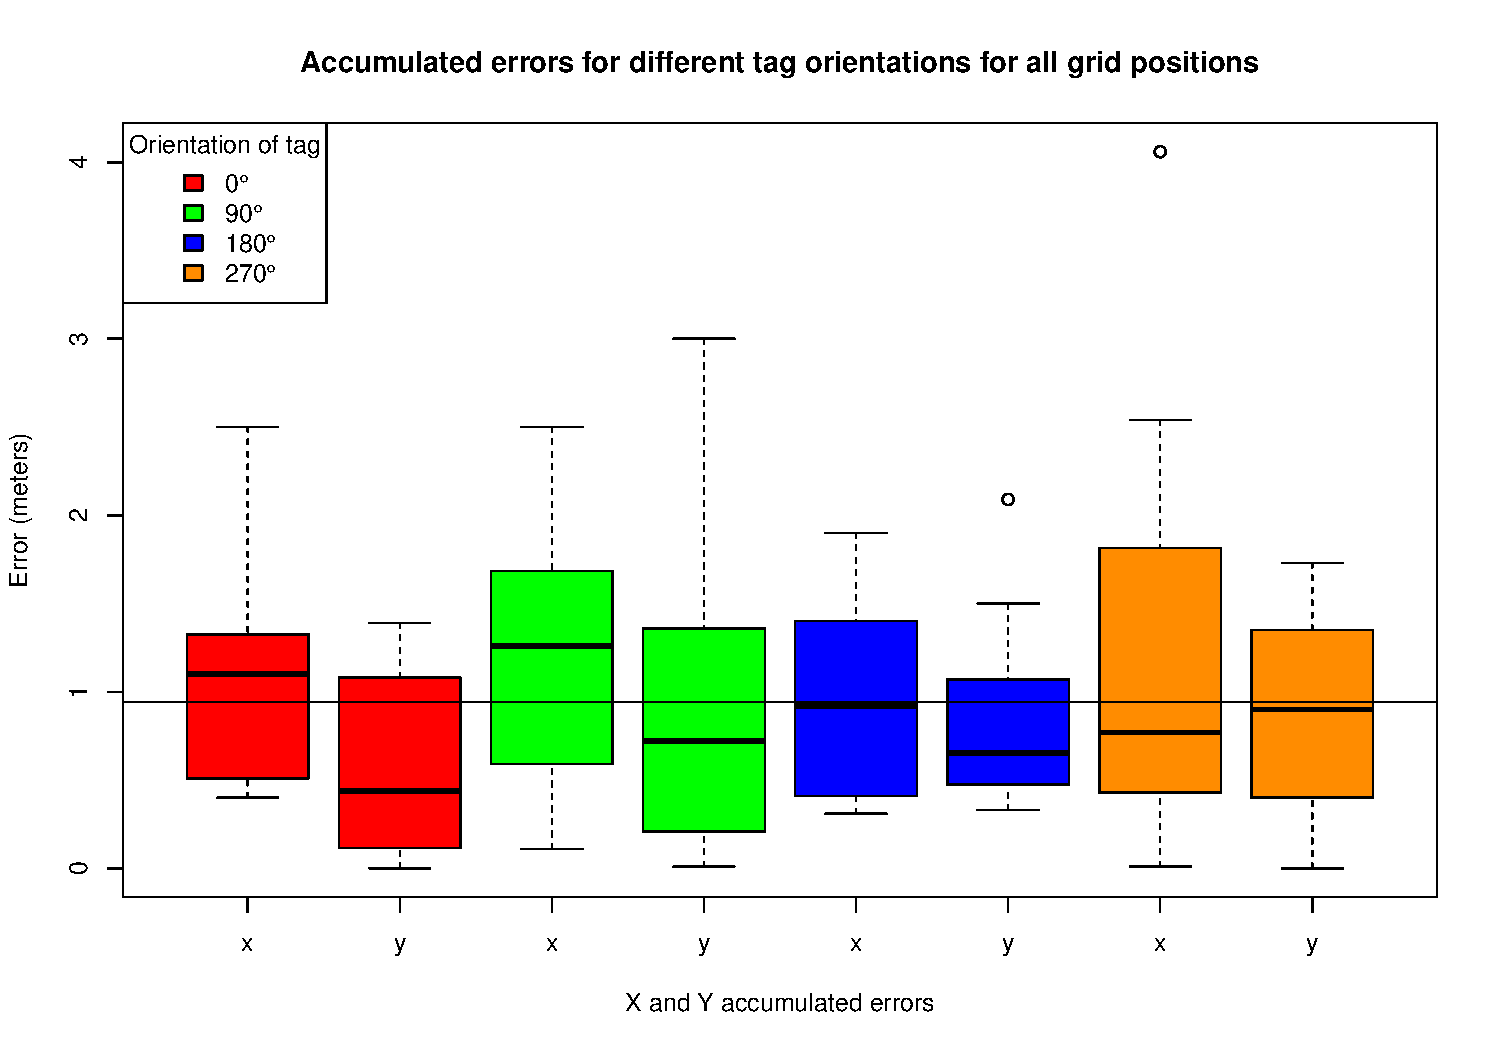
\includegraphics[width=.8\textwidth]{figures/error_boxplot}
		\caption{A box plot showing errors between measured and estimated locations. The boxes are organised in four groups. Each group consists of errors in $x$ and $y$ for a particular orientation of the tag. The horizontal line across the plot is the mean (0.943) of all errors regardless of the tag orientation.}
		\label{fig:errorlosbox}
	\end{center}
\end{figure}

In general, by looking at a plot for a certain position, one could tell the overall amount of error. Using this approach, it is evident that the system was localising the tag with a sub meter accuracy when the tag was placed equidistantly from the three readers. In positions where the tag was close to one reader but far from the other receivers, the system seemed to perform worse. The reason for this is in the way RSSI is converted to distance, rather the performance of the localisation algorithm. Section \ref{subsec:transtbl}, discussed a drawback of the translation tables. As the distance grows, RSSI values decrease at a slower rate. For example, for distances between zero and one meters, the second reader would measure 14 different RSSI values. In contrast, if the tag is five to six meters away, the RSSI changes by one unit (data from Appendix \ref{sec:trans}). Consequently, as distance increases, the accuracy of the RSSI to distance conversion decreases.

Figure \ref{fig:errorlosbox} is an alternative visualisation of the experimental results. It is a plot of the errors in $x$ and $y$ grouped by orientation disregarding the position of the tag on the grid. The plot shows that different orientations produce various amounts of error. For instance, when the tag was facing to the left (180\textdegree) in all positions, the mean error was under one meter in both $x$ and $y$. This figure also contains a horizontal line marking the average error (0.943m) of all measurements of this experiment.


\subsection{Three-dimensional grid of positions}
\label{sec:3d}

The purpose of this experiment was to test the localisation performance of the system in a three-dimensional setting. In a university computer laboratory, a space, that was four meters wide, six meters long, and two meters high, was selected. The walls of the room were lined with desks, chairs, and computers. One of the corners, where desks met, was marking the start of the coordinate system used by the system. The reader nodes were positioned on the sides of this space. They were also elevated at three different heights from the room floor. The first reader was set up at 2.4 meters to the right and 1.7 meters above ground from the point marking the origin. The second reader had the following coordinates (3.4m , 5.7m , 0.75m), which was the furthest from the origin and its receiver was placed on a table. The last reader was 3.2 meters down from the start of the coordinate system and eight centimetres above the floor.

After the readers were set up, the tag was repeatedly moved in a three-dimensional grid of positions. The $x$ and $y$ coordinates of the grid were starting half a meter from the origin in order to avoid obstacles that were in the way of the stand, used to lift the tag off the floor. The three heights at which the readers were positioned determined the $z$ component of the grid. This experimental setup is visualised on Figure \ref{fig:lastgrid}. It shows the positions of the readers and tag.

In order to produce a three-dimensional position for the tag, the system had to be modified slightly. Section \ref{sec:trilatmeth} described how trilateration worked. In three dimensions, the number of solutions is determined by the $z$ component. In rare cases when the sphere surfaces touch in one point, there is a single solution to the positioning problem. In most cases, however, the three spheres intersect, which results in two points of intersection, as shown on Figure \ref{fig:inter}. In this experiment, the middle point of the line segment formed by the two intersection points was used as the estimated position of the tag. Then, it was subtracted from the real position of the tag, manually inputted into the system. This gave the localisation error in three dimensions:
\[error = (|x_{real} - \frac{x_1 + x_2}{2}|, \ |y_{real} - \frac{y_1 + y_2}{2}|, \ |z_{real} - \frac{z_1 + z_2}{2}|)\]
\begin{figure}[H]
	\begin{center}
		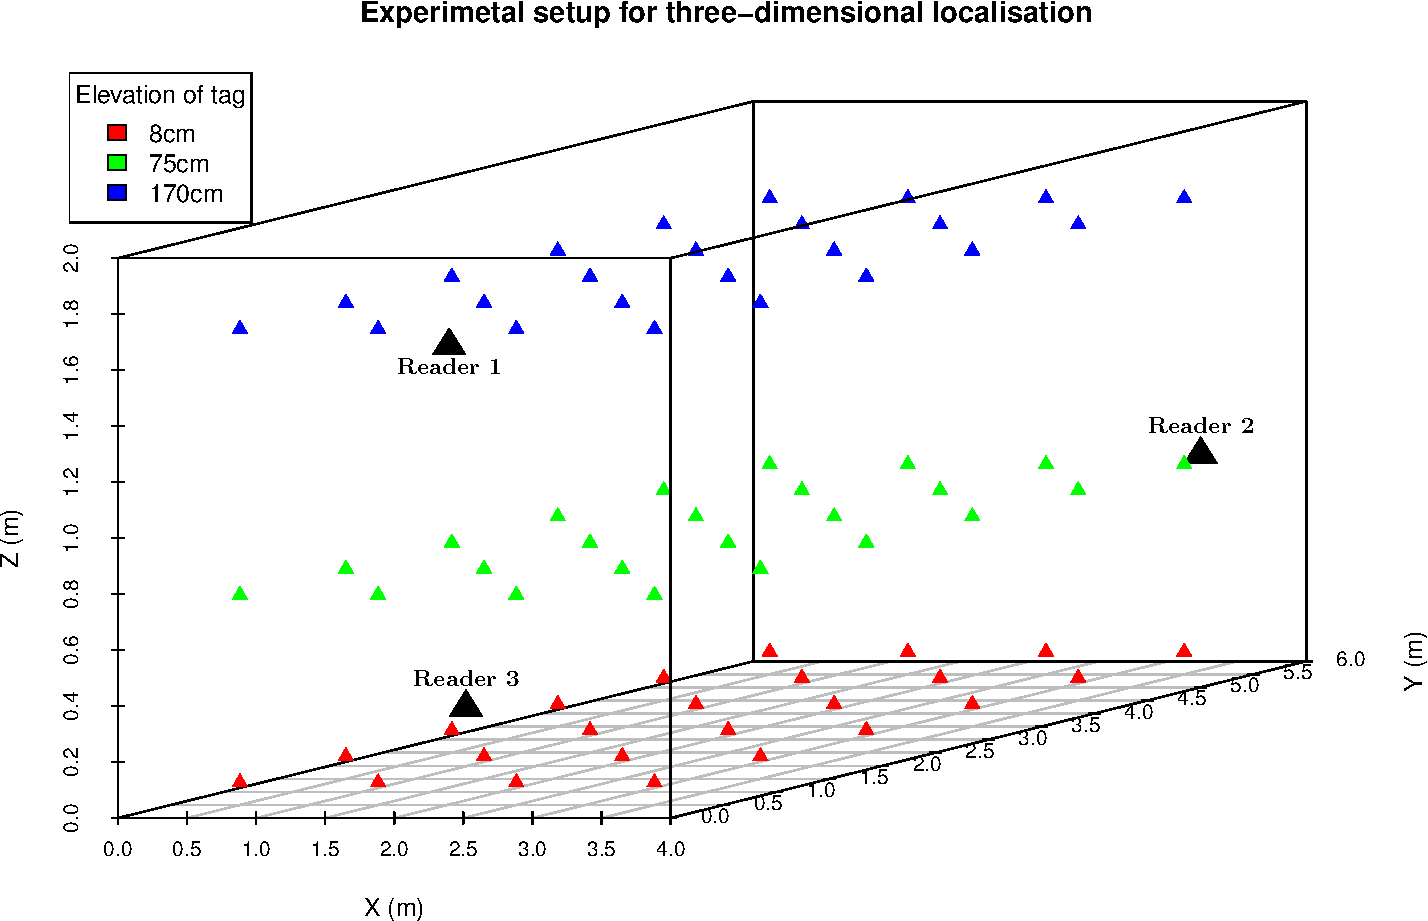
\includegraphics[width=1\textwidth]{figures/grid}
		\caption{Experimental setup for testing the localisation system in three dimensions. The positions of the readers are shown as black triangles. Their coordinates are (2.4, 0.0, 1.7), (3.4, 5.7, 0.75), and (0.0, 3.2, 0.08). Three tag elevations are marked by colours to visualise the grid of positions better.}
		\label{fig:lastgrid}
	\end{center}
\end{figure}
\begin{figure}[H]
	\begin{center}
		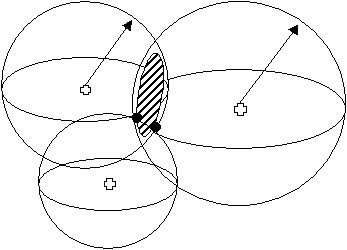
\includegraphics[width=.35\textwidth]{figures/intersect}
		\caption{The intersection of two spheres is a circle. A third sphere narrows down the intersection to two points\protect\footnotemark.}
		\label{fig:inter}
	\end{center}
\end{figure}
\footnotetext{Global Positioning System - \url{http://pegasus.cc.ucf.edu/~jweisham/pcb5937/GPS/GPS.html}.}

The results from this experiment are plotted on figures \ref{fig:errorbox3d} and \ref{fig:errortall}. Figure \ref{fig:errorbox3d} is a plot of the errors in $x$, $y$, and $z$ for every elevation of the tag from the room floor. The data was visualised in this way in order to investigate which horizontal plane in a room provides the best propagation medium. The first three boxes in the plot illustrate the three-dimensional localisation error for the positions of the tag when it was eight centimetres from the ground. It can be seen that the spread of the errors in both $x$ and $y$ was significant, although its mean was close to one meter. The reason for this might be that there are a lot of obstacles in the lower parts of an indoor space, such as chairs and tables. These objects decrease the signal strength of the radio signal emitted from the tag. Another factor is the vertical distance between a reader and transmitter. Looking at diagram \ref{fig:ele} used in a previous experiment, it is evident that radio signals have to travel greater distances to reach receivers positioned at a different height.
\begin{figure}[H]
	\begin{center}
		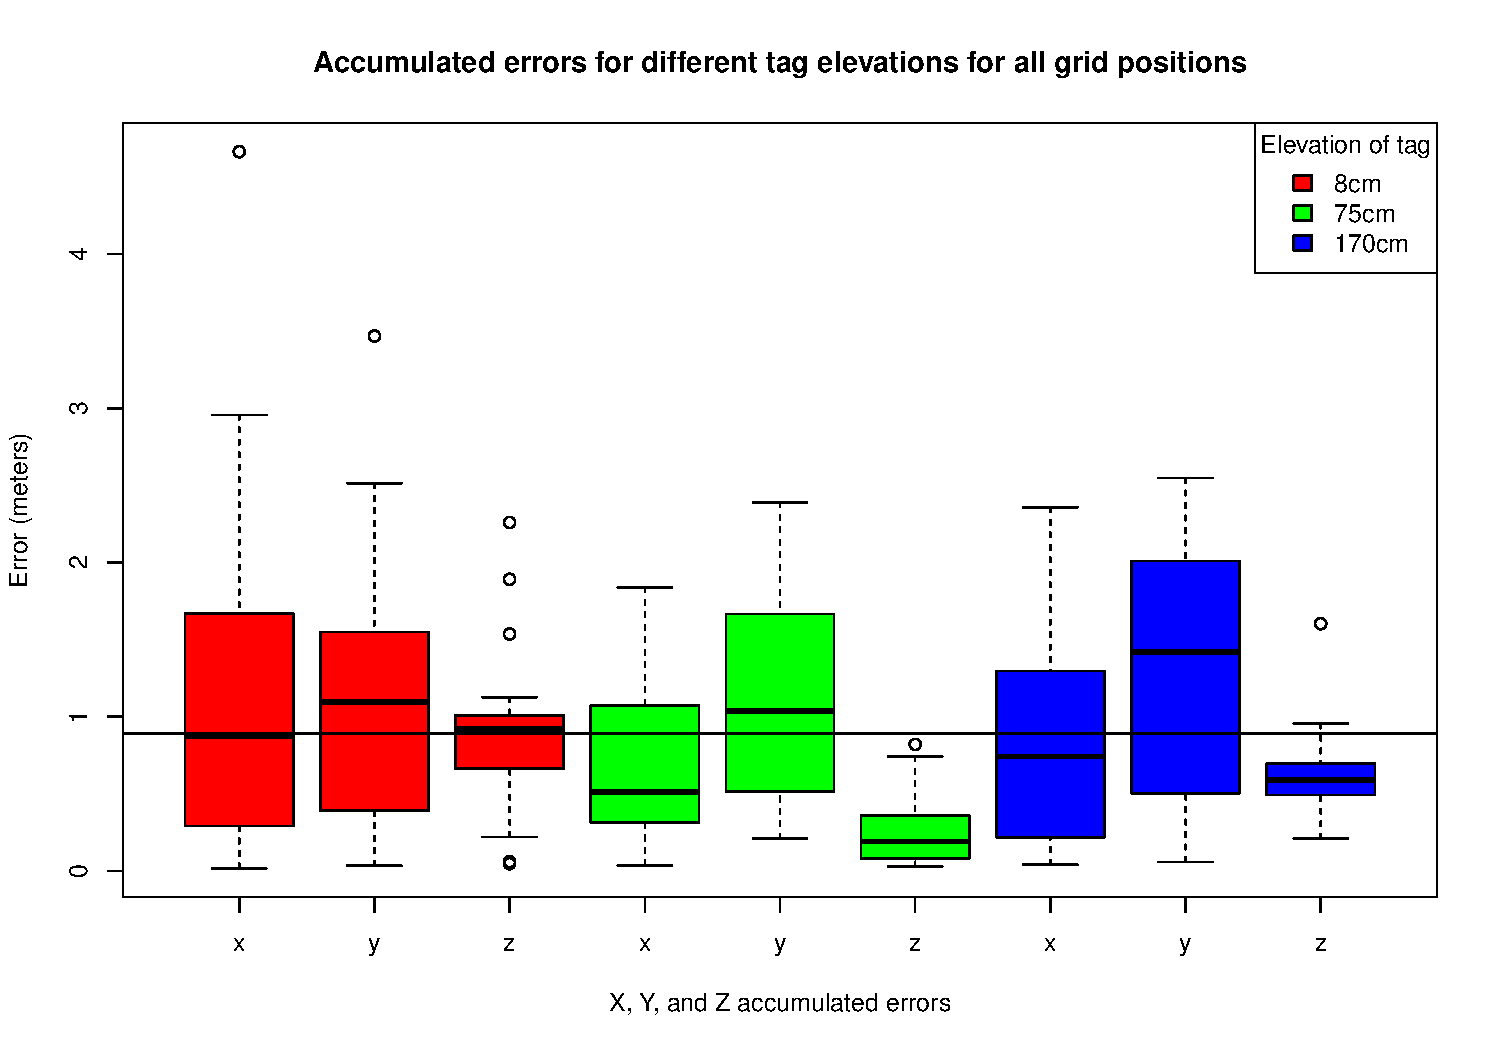
\includegraphics[width=.8\textwidth]{figures/error_boxplot_3d}
		\caption{A box plot showing errors between measured and estimated locations. The boxes are organised in three groups. Each group consists of errors in the $x$, $y$, and $z$ for a particular elevation of the tag. The horizontal line across the plot is the mean (0.8895182) of all errors regardless of the tag elevation.}
		\label{fig:errorbox3d}
	\end{center}
\end{figure}
The same reasoning can be applied to the case when the tag was high above ground (170cm). The last three columns of figure \ref{fig:errorbox3d} show the distribution of the localisation error for this elevation. Again, the errors in $x$ and $y$ had a substantial spread. The error in $z$ appeared to be low regardless of the elevation. Although, the upper parts of an indoor space are usually free from obstacles, this experiment showed that the system produced a considerable localisation error. By placing the tag at desk level (75cm), the system demonstrated the least deviation from the real positions of the tag. A possible explanation is that the tag was in the middle of the grid of positions, which enabled it to be read from below, middle, and above. These RSSI values provided a better estimation of the distance between the devices.
\begin{figure}[H]
	\begin{center}
		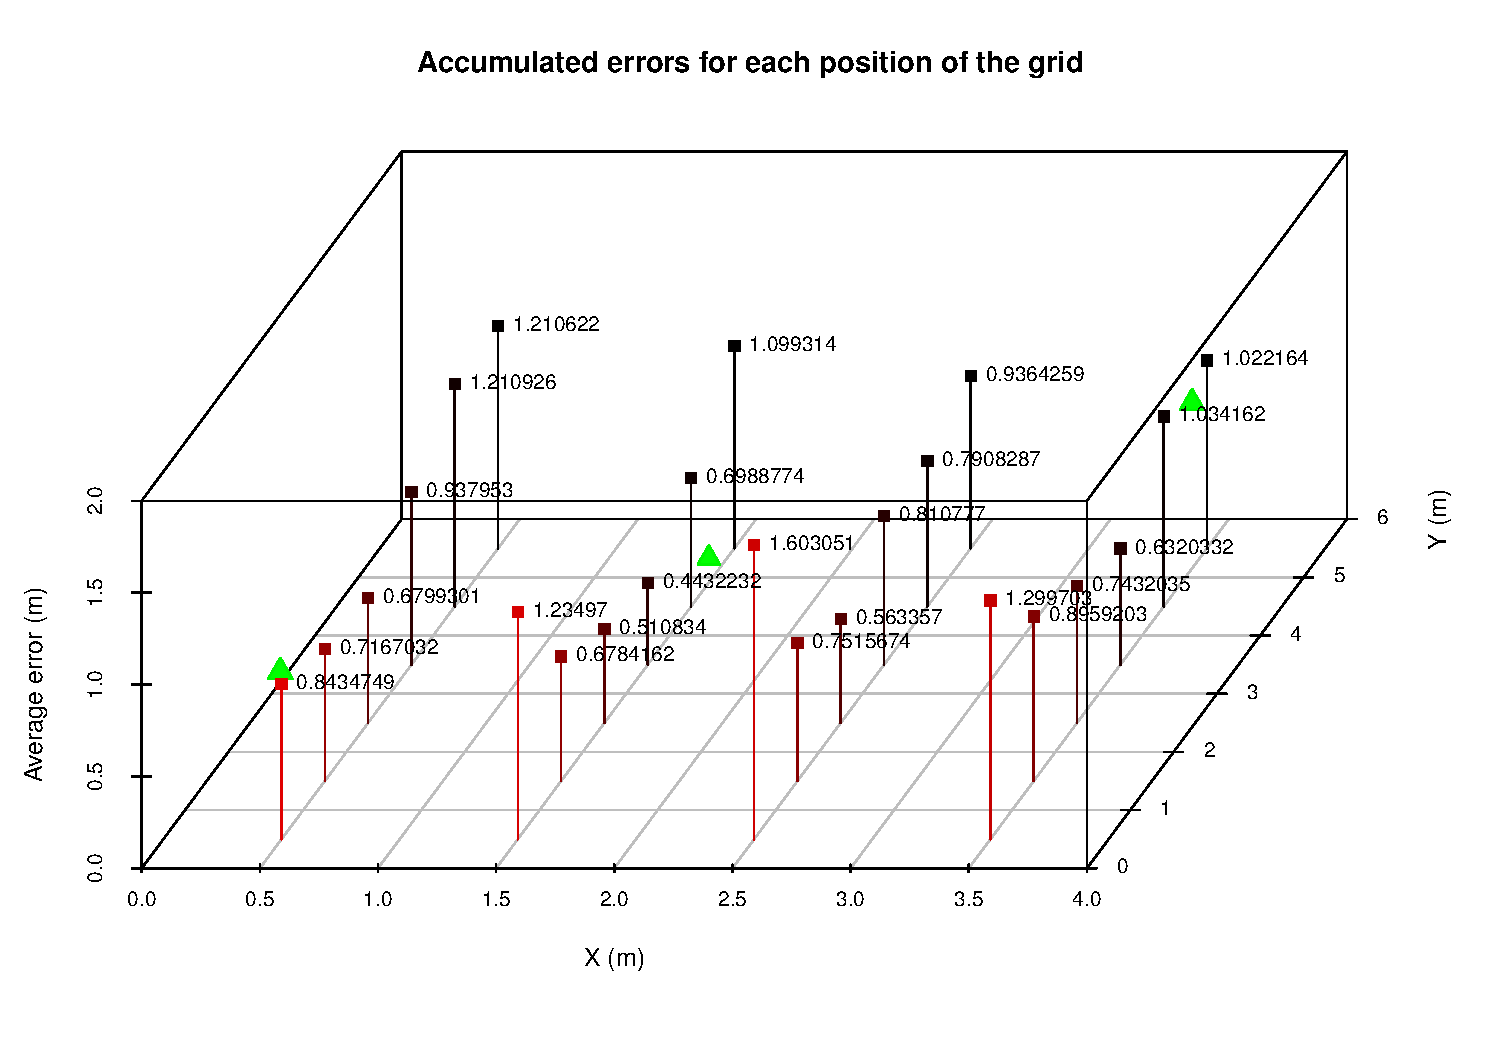
\includegraphics[width=1\textwidth]{figures/tall2}
		\caption{A three-dimensional scatter plot of the average error for every position in the grid regardless of the elevation of the tag. The $x$ and $y$ axes are the coordinates of the space and the $z$-axis is the average error in meters. The numbers to the right of every position are the mean errors. Three green triangles mark the positions of the readers, which are on the front, back, and left faces of the rectangular parallelepiped.}
		\label{fig:errortall}
	\end{center}
\end{figure}

Figure \ref{fig:errortall} is a three-dimensional scatter plot of the mean error for every position in the grid regardless of the elevation of the tag. This data visualisation shows the places where the system estimated the location of the tag with a certain accuracy. Recall that the walls of this indoor environment were lined with objects and that the readers were set up at three of the sides of the test space. These obstacles were a contributing factor that increased the localisation error at the boundaries of the grid. Similar to the results of the previous experiment, lower errors were observed in the central parts of the grid, where tag was at similar distances from the receivers. When the transmitter was close to one but far from the other readers, the errors spiked due to inaccuracies in the conversion from RSSI to distance as the gap between devices increased.

In this experiment, the mean error of all positions in the grid was 0.89 meters. It was brought down mainly due to the low localisation errors of the $z$ component. Although the overall error was low, the system computed locations that were usually off by at least a meter in one dimension. In a real situation, this means that a person searching for an object tagged with a transmitter has to scan a spherical area determined by the amount of error to locate the object's true position.

\section{Discussion}

This section provides a discussion of the system's performance. In particular, the outcomes from the hardware evaluation are summarised. Then, the results of the experiments with the system are analysed and compared to the related work. Finally, potential applications of the system are described.

\subsection{RFID Hardware}

The RFID devices used in this project had a very affordable price. They provided a great value for money. The receivers had an RSSI module and the tag was emitting a strong signal. The range of the system was bigger than advertised  (13m). The readers could also detect the transmitter through walls.

Nevertheless, there were a number of disadvantages. First, the receivers were not calibrated to each other, which resulted in different RSSI measurements for equal distances. Second, the resolution of the RSSI modules was smaller than expected, which had a serious impact on the localisation accuracy of the system. Third, RSSI values were often changing unpredictably as distance grew. In addition, the battery of the tag was a factor contributing to the variations of the RSSI measurements.

A number of observations were made during the experimentation with the hardware. Generally, if the readers had a line of sight to the tag, the RSSI readings were more reliable compared to cases when the receivers were facing away from the transmitter. In addition, the placement of the devices in an indoor space determined the quality of the localisation. As it was found in section \ref{sec:3d}, the best elevation for a tag was above office furniture or other types of obstacles. The positions of the readers in a three-dimensional space also played a role in the behaviour of the system. Placing the readers too high or too low in a room, introduced errors in the distance estimation. Also, setting up the reader nodes in corners did not cover long stretches of indoor space. Consequently, potential spots were desks near walls with a good view of the whole area.

\subsection{Localisation performance}

The performance of the system in terms of localisation accuracy was tested in two experiments. The first was conducted in two dimensions and checked whether rotating the tag around its base had any effect on the evaluation metric. The second experiment was resembling a potential application scenario of the system. It was carried out in a larger three-dimensional space with office furniture. The results of these experiments can be summarised into mean localisation errors in meters between the computed and true positions of the transmitter. The experiments achieved average errors of 0.943 and 0.889, respectively. There are many experimental cases that were not tested in this project. These might increase the mean localisation error of the system. For instance, scenarios with people, robots, or vehicles moving through the environment could seriously influence the RSSI measurements of the receivers. Moreover, this project did not test placing the receiver in adjacent rooms or floors of a building. Nonetheless, the above experiments gave a rough idea of the system capabilities.

Compared to the previous work in this research field, the location sensing system of this project was closest to the SpotON system, described in section \ref{sec:spoton}. Both systems estimated locations in three dimensions, used received signal strength to compute distance, and relied on the lateration geometrical method. The SpotON system achieved accuracy of three meters with hardware providing a limited RSS resolution. The authors developed a custom hardware that reported sub meter localisation accuracy. Similar localisation error was measured in this project. In contrast, this system used affordable single-board computers that had substantial processing power and were very portable. Moreover, the RFID hardware of this project had a better RSSI sensitivity.

The LANDMARC system, presented in section \ref{sec:landmarc}, can be also compared with this system. LANDMARC had a different approach and was a two-dimensional location system. It was employing a grid of reference RFID tags that were used as neighbours to the tracked tag. The k-nearest neighbours were the basis for estimating the location of the unknown tag. The authors had hardware issues that were not encountered in this project. For instance, their hardware did not supply received signal strength directly. Their system achieved average distance error of one meter, which is similar to the results in this project. LANDMARC uses reference tags as an additional infrastructure, which is an important advantage over this system. The reference tags were subject to the same physical conditions as the tracked tags. This means that if there was a big occlusion between the readers and transmitters, the reference tags would be used to minimise the severe effects on the radio signals caused by big obstacles. Nevertheless, this technique required extra RFID tags, which had batteries and needed to be set up in a grid occupying extra space. In contrast, the system of this project were very portable (fitted in a backpack) and could be installed in minutes. Furthermore, having multiple processing nodes provided interesting opportunities to add functionality on top of location sensing. One example used in this project was providing a web interface to remotely control and monitor the system. Utilisation of the processing power of the computers is discussed in section \ref{sec:future}.

\subsection{Applications}

There are many scenarios where this location sensing system can be applied. Generally, the RFID technology is mainly used for identification purposes. It has applications in supply chain and asset management, health services, and in the military, to name a few. Adding a location context to the identity of an object is a big plus. In addition to the applications of the technology discussed in section \ref{sec:rfidapp}, this system can be used to localise expensive hospital equipment or track patients. It can be used for robot navigation in indoor spaces if attached to agents. Locating an important parcel in a warehouse can become easier using this system. Visitors of a conference could wear the transmitters as badges in order to track their movement and analyse their interaction patterns\footnote{OpenAMD Project - \url{http://www.openamd.org/}}.

In the spectrum of location accuracy and precision, this system can definitely sense the presence of a tag if it is in range. Having achieved an average localisation accuracy of around one meter, the system is a viable candidate for the above scenarios. However, the current system cannot be used for very precise localisation due to the disadvantages of the RFID hardware used in this project. Even if expensive devices are used, it can be the case that RSSI is an unreliable metric for estimating distance, as some researchers have argued \cite{Elnahrawy2004, Parameswaran2009}.


\section{Summary}

This chapter presented the experiments conducted to evaluate the RFID hardware and localisation accuracy of the system. Section \ref{sec:hardeval} described tests of the RFID hardware. Then, section \ref{sec:syseval} detailed the experiments that checked how the system performed in terms of localisation accuracy. Next, these results were compared to of the ones of related work. Finally, some potential applications of the system were discussed. The next chapter concludes this work, detailing its contributions and describing what can be done in the future.
